\documentclass[]{book}
\usepackage{lmodern}
\usepackage{amssymb,amsmath}
\usepackage{ifxetex,ifluatex}
\usepackage{fixltx2e} % provides \textsubscript
\ifnum 0\ifxetex 1\fi\ifluatex 1\fi=0 % if pdftex
  \usepackage[T1]{fontenc}
  \usepackage[utf8]{inputenc}
\else % if luatex or xelatex
  \ifxetex
    \usepackage{mathspec}
  \else
    \usepackage{fontspec}
  \fi
  \defaultfontfeatures{Ligatures=TeX,Scale=MatchLowercase}
\fi
% use upquote if available, for straight quotes in verbatim environments
\IfFileExists{upquote.sty}{\usepackage{upquote}}{}
% use microtype if available
\IfFileExists{microtype.sty}{%
\usepackage{microtype}
\UseMicrotypeSet[protrusion]{basicmath} % disable protrusion for tt fonts
}{}
\usepackage[margin=1in]{geometry}
\usepackage{hyperref}
\hypersetup{unicode=true,
            pdftitle={Panduan Pemasangan dan Penggunaan R dan ggplot2},
            pdfauthor={Wihelmus Wedo},
            pdfborder={0 0 0},
            breaklinks=true}
\urlstyle{same}  % don't use monospace font for urls
\usepackage{natbib}
\bibliographystyle{apalike}
\usepackage{color}
\usepackage{fancyvrb}
\newcommand{\VerbBar}{|}
\newcommand{\VERB}{\Verb[commandchars=\\\{\}]}
\DefineVerbatimEnvironment{Highlighting}{Verbatim}{commandchars=\\\{\}}
% Add ',fontsize=\small' for more characters per line
\usepackage{framed}
\definecolor{shadecolor}{RGB}{248,248,248}
\newenvironment{Shaded}{\begin{snugshade}}{\end{snugshade}}
\newcommand{\KeywordTok}[1]{\textcolor[rgb]{0.13,0.29,0.53}{\textbf{#1}}}
\newcommand{\DataTypeTok}[1]{\textcolor[rgb]{0.13,0.29,0.53}{#1}}
\newcommand{\DecValTok}[1]{\textcolor[rgb]{0.00,0.00,0.81}{#1}}
\newcommand{\BaseNTok}[1]{\textcolor[rgb]{0.00,0.00,0.81}{#1}}
\newcommand{\FloatTok}[1]{\textcolor[rgb]{0.00,0.00,0.81}{#1}}
\newcommand{\ConstantTok}[1]{\textcolor[rgb]{0.00,0.00,0.00}{#1}}
\newcommand{\CharTok}[1]{\textcolor[rgb]{0.31,0.60,0.02}{#1}}
\newcommand{\SpecialCharTok}[1]{\textcolor[rgb]{0.00,0.00,0.00}{#1}}
\newcommand{\StringTok}[1]{\textcolor[rgb]{0.31,0.60,0.02}{#1}}
\newcommand{\VerbatimStringTok}[1]{\textcolor[rgb]{0.31,0.60,0.02}{#1}}
\newcommand{\SpecialStringTok}[1]{\textcolor[rgb]{0.31,0.60,0.02}{#1}}
\newcommand{\ImportTok}[1]{#1}
\newcommand{\CommentTok}[1]{\textcolor[rgb]{0.56,0.35,0.01}{\textit{#1}}}
\newcommand{\DocumentationTok}[1]{\textcolor[rgb]{0.56,0.35,0.01}{\textbf{\textit{#1}}}}
\newcommand{\AnnotationTok}[1]{\textcolor[rgb]{0.56,0.35,0.01}{\textbf{\textit{#1}}}}
\newcommand{\CommentVarTok}[1]{\textcolor[rgb]{0.56,0.35,0.01}{\textbf{\textit{#1}}}}
\newcommand{\OtherTok}[1]{\textcolor[rgb]{0.56,0.35,0.01}{#1}}
\newcommand{\FunctionTok}[1]{\textcolor[rgb]{0.00,0.00,0.00}{#1}}
\newcommand{\VariableTok}[1]{\textcolor[rgb]{0.00,0.00,0.00}{#1}}
\newcommand{\ControlFlowTok}[1]{\textcolor[rgb]{0.13,0.29,0.53}{\textbf{#1}}}
\newcommand{\OperatorTok}[1]{\textcolor[rgb]{0.81,0.36,0.00}{\textbf{#1}}}
\newcommand{\BuiltInTok}[1]{#1}
\newcommand{\ExtensionTok}[1]{#1}
\newcommand{\PreprocessorTok}[1]{\textcolor[rgb]{0.56,0.35,0.01}{\textit{#1}}}
\newcommand{\AttributeTok}[1]{\textcolor[rgb]{0.77,0.63,0.00}{#1}}
\newcommand{\RegionMarkerTok}[1]{#1}
\newcommand{\InformationTok}[1]{\textcolor[rgb]{0.56,0.35,0.01}{\textbf{\textit{#1}}}}
\newcommand{\WarningTok}[1]{\textcolor[rgb]{0.56,0.35,0.01}{\textbf{\textit{#1}}}}
\newcommand{\AlertTok}[1]{\textcolor[rgb]{0.94,0.16,0.16}{#1}}
\newcommand{\ErrorTok}[1]{\textcolor[rgb]{0.64,0.00,0.00}{\textbf{#1}}}
\newcommand{\NormalTok}[1]{#1}
\usepackage{longtable,booktabs}
\usepackage{graphicx,grffile}
\makeatletter
\def\maxwidth{\ifdim\Gin@nat@width>\linewidth\linewidth\else\Gin@nat@width\fi}
\def\maxheight{\ifdim\Gin@nat@height>\textheight\textheight\else\Gin@nat@height\fi}
\makeatother
% Scale images if necessary, so that they will not overflow the page
% margins by default, and it is still possible to overwrite the defaults
% using explicit options in \includegraphics[width, height, ...]{}
\setkeys{Gin}{width=\maxwidth,height=\maxheight,keepaspectratio}
\IfFileExists{parskip.sty}{%
\usepackage{parskip}
}{% else
\setlength{\parindent}{0pt}
\setlength{\parskip}{6pt plus 2pt minus 1pt}
}
\setlength{\emergencystretch}{3em}  % prevent overfull lines
\providecommand{\tightlist}{%
  \setlength{\itemsep}{0pt}\setlength{\parskip}{0pt}}
\setcounter{secnumdepth}{5}
% Redefines (sub)paragraphs to behave more like sections
\ifx\paragraph\undefined\else
\let\oldparagraph\paragraph
\renewcommand{\paragraph}[1]{\oldparagraph{#1}\mbox{}}
\fi
\ifx\subparagraph\undefined\else
\let\oldsubparagraph\subparagraph
\renewcommand{\subparagraph}[1]{\oldsubparagraph{#1}\mbox{}}
\fi

%%% Use protect on footnotes to avoid problems with footnotes in titles
\let\rmarkdownfootnote\footnote%
\def\footnote{\protect\rmarkdownfootnote}

%%% Change title format to be more compact
\usepackage{titling}

% Create subtitle command for use in maketitle
\providecommand{\subtitle}[1]{
  \posttitle{
    \begin{center}\large#1\end{center}
    }
}

\setlength{\droptitle}{-2em}

  \title{Panduan Pemasangan dan Penggunaan R dan ggplot2}
    \pretitle{\vspace{\droptitle}\centering\huge}
  \posttitle{\par}
    \author{Wihelmus Wedo}
    \preauthor{\centering\large\emph}
  \postauthor{\par}
      \predate{\centering\large\emph}
  \postdate{\par}
    \date{2019-06-17}

\usepackage{booktabs}
\usepackage[bahasai]{babel}

\usepackage{fontspec}
\setmainfont{Linux Libertine O}
\setmonofont{SauceCodePro Nerd Font}

\usepackage{setspace}

\onehalfspacing

\begin{document}
\maketitle

{
\setcounter{tocdepth}{1}
\tableofcontents
}
\chapter*{Kata Pengantar}\label{kata-pengantar}
\addcontentsline{toc}{chapter}{Kata Pengantar}

Selama ini penulis mengamati bahwa grafik dalam publikasi BPS biasanya
dibuat dalam perangkat lunak \emph{Microsoft Office Excel} (MS Excel).
Aplikasi ini telah banyak digunakan oleh banyak orang dan berbasis
\emph{Graphical User Interface}. Penulis merasa bahwa grafik yang dibuat
dapat ditingkatkan efektivitas dan efisiensinya. Penulis -- seseorang
yang telah belajar tentang R sewaktu kuliah -- ingin mengaplikasikan R
dan ggplot2 pada pekerjaannya. Penulis menyadari bahwa untuk membuat
grafik yang efektif, seseorang bisa saja menggunakan program seperti
\emph{Microsoft Office Excel}. Akan tetapi terdapat beberapa hambatan
ketika menggunakan 3, diantaranya

\begin{enumerate}
\def\labelenumi{\arabic{enumi}.}
\tightlist
\item
  Menghabiskan waktu relatif lama untuk membuat grafik yang efektif
\item
  Sejatinya, seseorang harus membayar untuk menggunakan MS Excel.
\item
  Proses yang sama perlu dilakukan berkali-kali seiring dengan
  pemutakhiran data.
\item
  Untuk membuka file Excel diperlukan MS Excel.
\end{enumerate}

Penulis merasa bahwa hal-hal tersebut dapat diminimalisasi dengan
menggunakan R dan ggplot2. R sebagai sebuah \emph{Free and Open Source
Software} (FOSS) bersifat \emph{gratis} dan \emph{bebas} sehingga siapa
pun dapat dengan mudah mengunduh, menggunakan, dan mengembangkan
perangkat lunak tersebut. Selain itu, \emph{Script} R hanyalah berbentuk
sebuah \emph{text file}. Hal tersebut memudahkan pengguna untuk
melakukan \emph{copy-paste} dan isinya dapat dibaca oleh \emph{text
editor} seperti Notepad, Neovim, Gedit, dll. Kemudahan untuk membuka dan
membaca \emph{script} R juga memiliki manfaat agar orang lain dapat
mengetahui proses pengerjaan suatu data dari awal dan akhir. Hal ini
mendorong terbentuknya \emph{reproducible analysis}.

Penulis dalam dokumen ini hanya sekadar membagi informasi mengenai
dasar-dasar penggunaan R, dan ggplot2. Dokumen ini \textbf{tidak
menjelaskan semua} hal mengenai R dan ggplot2 kepada pembaca. Akhir
kata, penulis ingin mengucapkan terima kasih kepada pembaca yang membaca
dokumen ini. Selamat membaca!

\chapter{Bahasa Pemrograman R}\label{R}

\section{Apa itu R?}\label{apa-itu-r}

\href{https://www.r-project.org/}{R} adalah sebuah bahasa pemrograman
yang digunakan untuk melakukan \emph{data analysis} atau \emph{data
science}. R diprakarsasi oleh Ross Ihaka dan Robert Gentleman sebagai
bentuk \emph{open source} dari S, salah satu bahasa pemrograman
statistik juga. Di masa kini, R banyak digunakan dalam hal \emph{data
science} atau \emph{data analysis} sebab sifatnya yang \emph{Free} dan
\emph{Open Source} memudahkan siapapun untuk membuat \emph{package}
untuk R. File R berbentuk \emph{script} atau \emph{text}. Bentuk ini
memudahkan pengguna R untuk mereproduksi atau replikasi dengan cara yang
sederhana (read: \emph{copy-paste}). Hadley Wickham -- salah satu orang
paling populer di dunia R -- membuat proses dilakukannya \emph{data
analysis} atau \emph{data science}. Salah satu proses tersebut adalah
visualisasi. Bentuk file R yang merupakan teks akan mempermudah proses
ini.

\section{Pemasangan R}\label{pemasangan-r}

\subsection*{Windows 10}\label{windows-10}
\addcontentsline{toc}{subsection}{Windows 10}

Cara terbaik untuk mengunduh R adalah dengan menggunakan situs resminya
yaitu \url{https://www.r-project.org/}. Dari situs tersebut, akan
diarahkan menuju \emph{mirror} terdekat. Indonesia memiliki mirror
terdekat yaitu milik Badan Pengkajian dan Penerapan Teknologi (BPPT).

\begin{enumerate}
\def\labelenumi{\arabic{enumi}.}
\tightlist
\item
  Untuk mempermudah, silahkan menuju tautan
  \url{https://repo.bppt.go.id/cran/}.
\item
  Setelah halaman terbuka, klik pada bagian \emph{Download R for
  Windows}
\item
  Kemudian akan muncul halaman baru, klik pada tautan \emph{base}
\item
  Setelah halaman baru muncul, klik pada tautan \emph{Download R 3.6.0
  for Windows}.
\item
  Setelah selesai mengunduh R, double pada file \emph{executable}
  (\emph{.exe}).
\end{enumerate}

Proses pemasangan R merupakan proses mudah, pembaca hanya perlu klik
tombol \emph{Next} atau \emph{OK} pada setiap jendela dialog.

\begin{figure}

{\centering 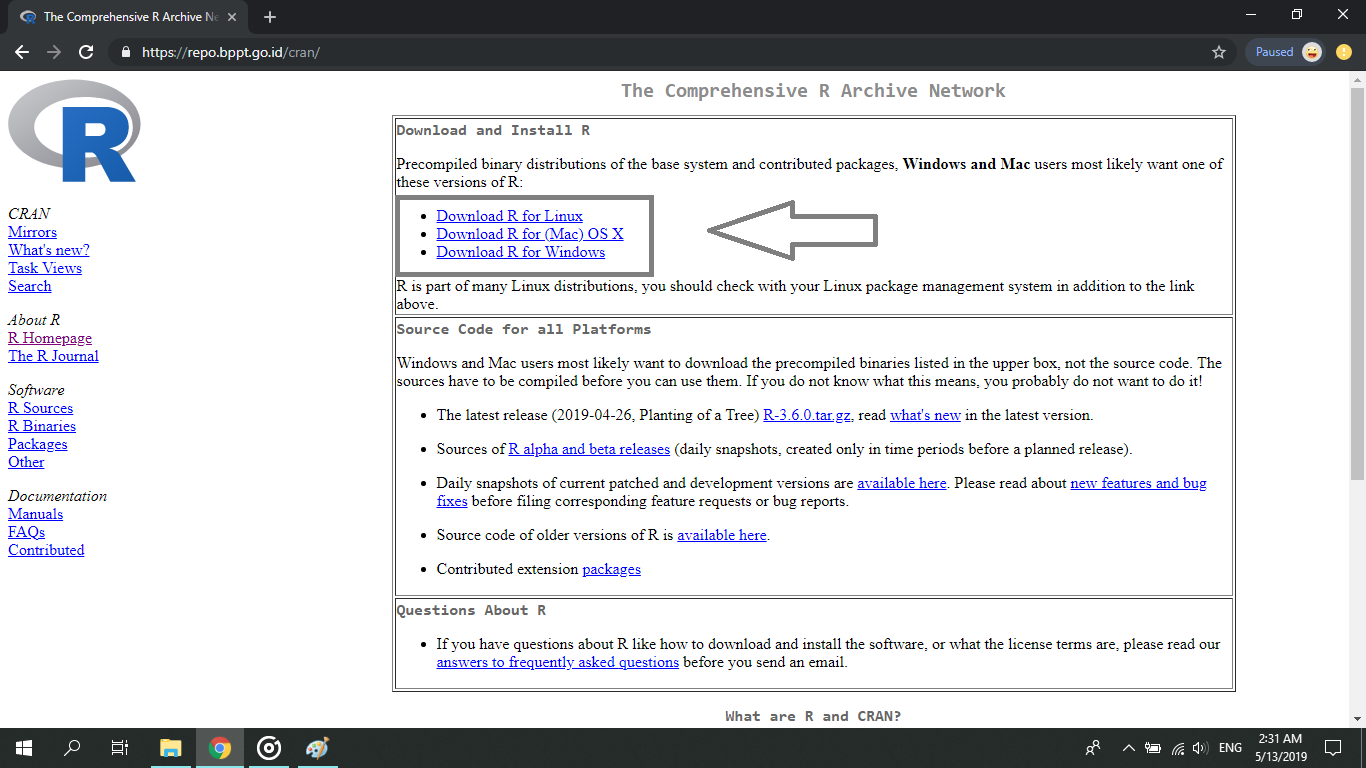
\includegraphics[width=0.9\linewidth]{Gambar/r-download/06} 

}

\caption{Repository R dari BPPT}\label{fig:install-r-1}
\end{figure}

\begin{figure}

{\centering 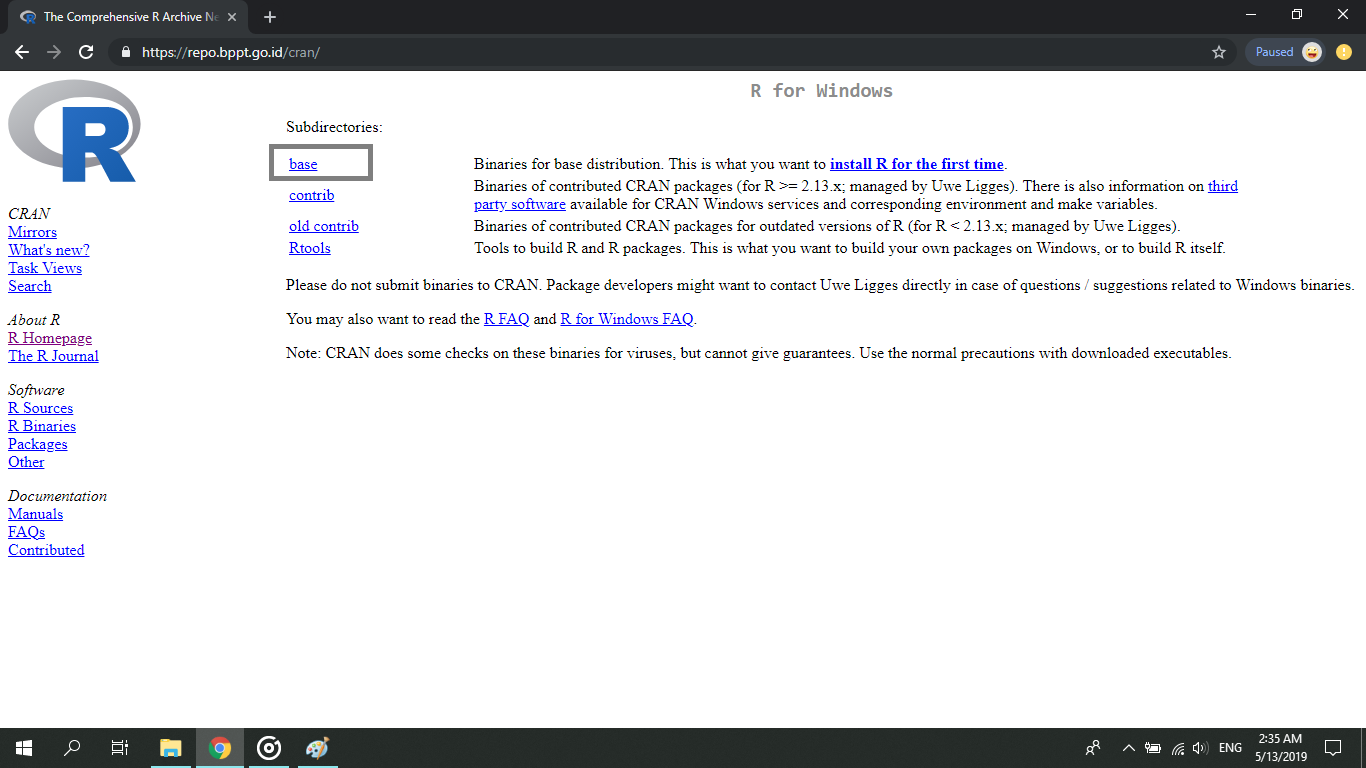
\includegraphics[width=0.9\linewidth]{Gambar/r-download/07} 

}

\caption{Klik pada tautan base}\label{fig:install-r-2}
\end{figure}

\begin{figure}

{\centering 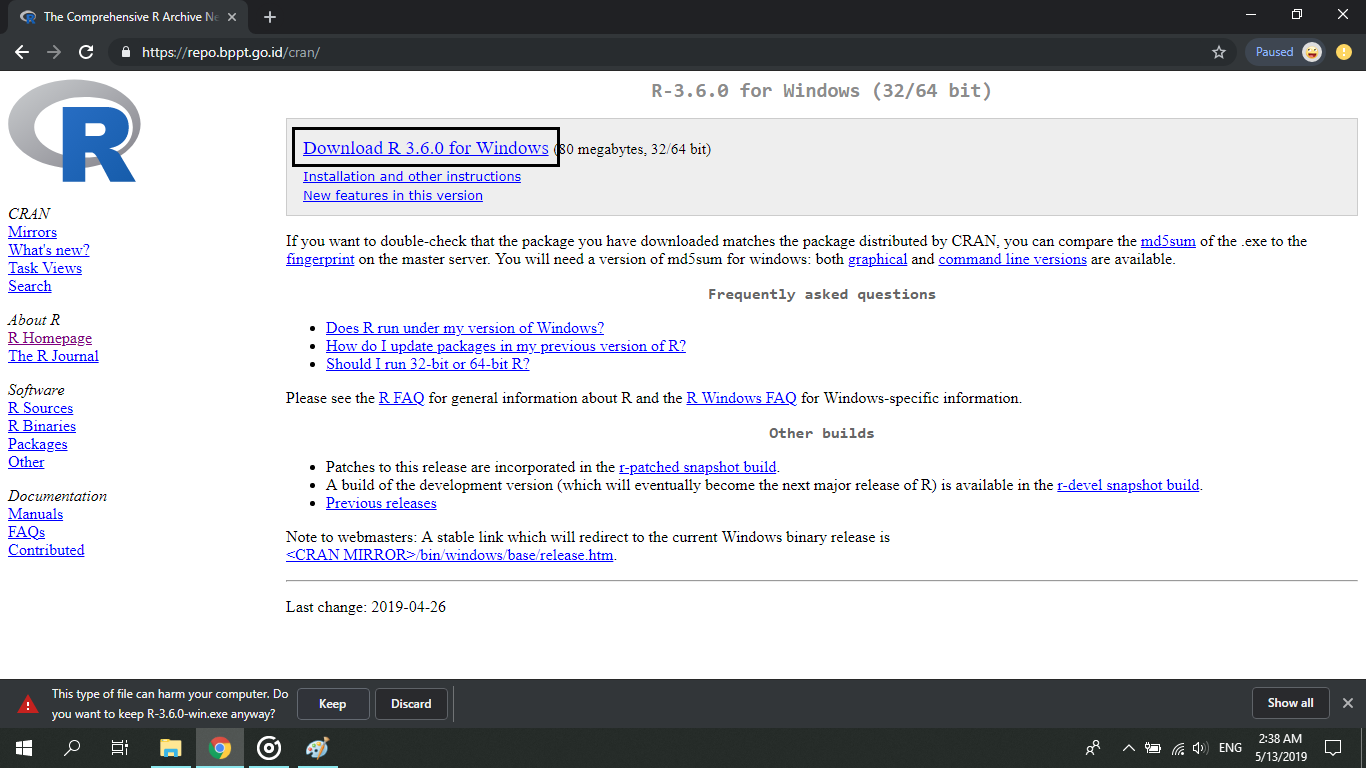
\includegraphics[width=0.9\linewidth]{Gambar/r-download/09} 

}

\caption{Klik pada Download R 3.6.0 for Windows}\label{fig:install-r-3}
\end{figure}

\begin{figure}

{\centering 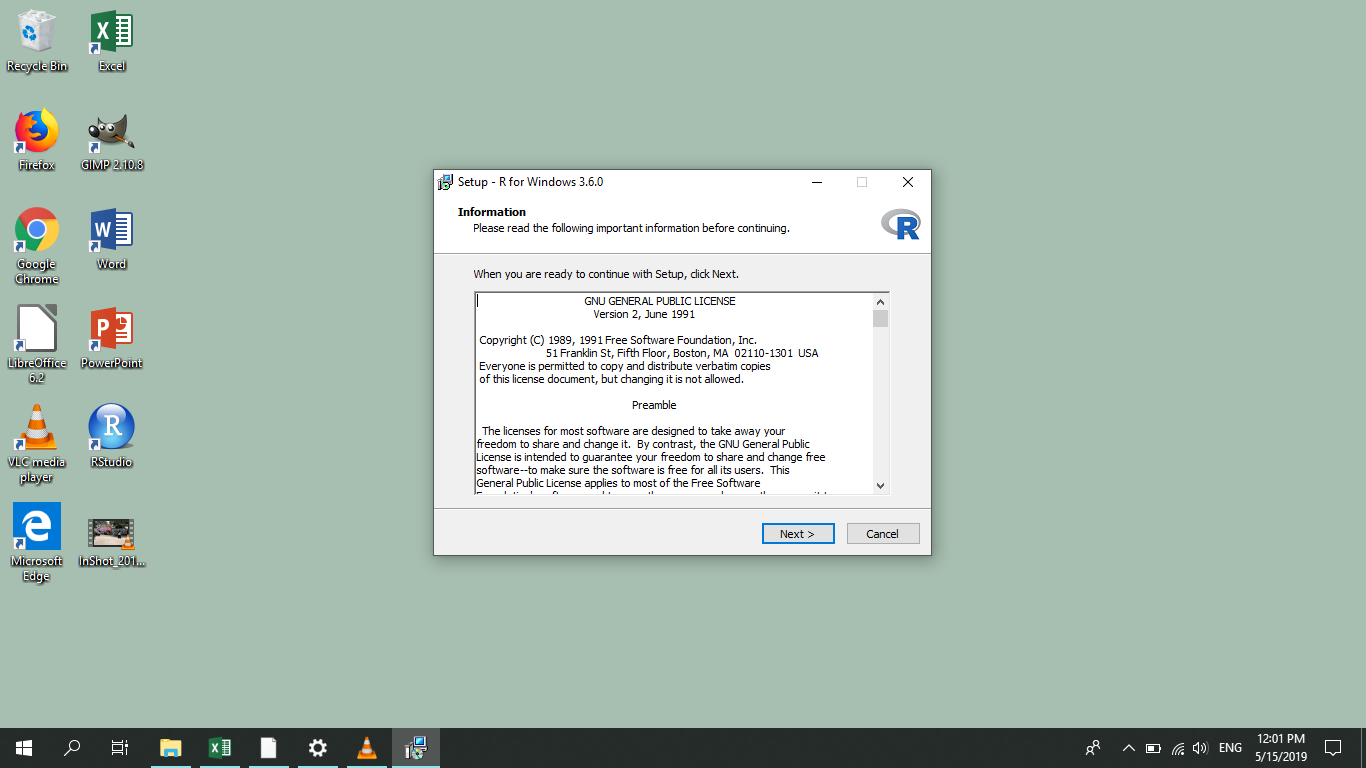
\includegraphics[width=0.9\linewidth]{Gambar/r-download/10} 

}

\caption{Kotak dialog untuk R}\label{fig:install-r-4}
\end{figure}

\begin{figure}

{\centering 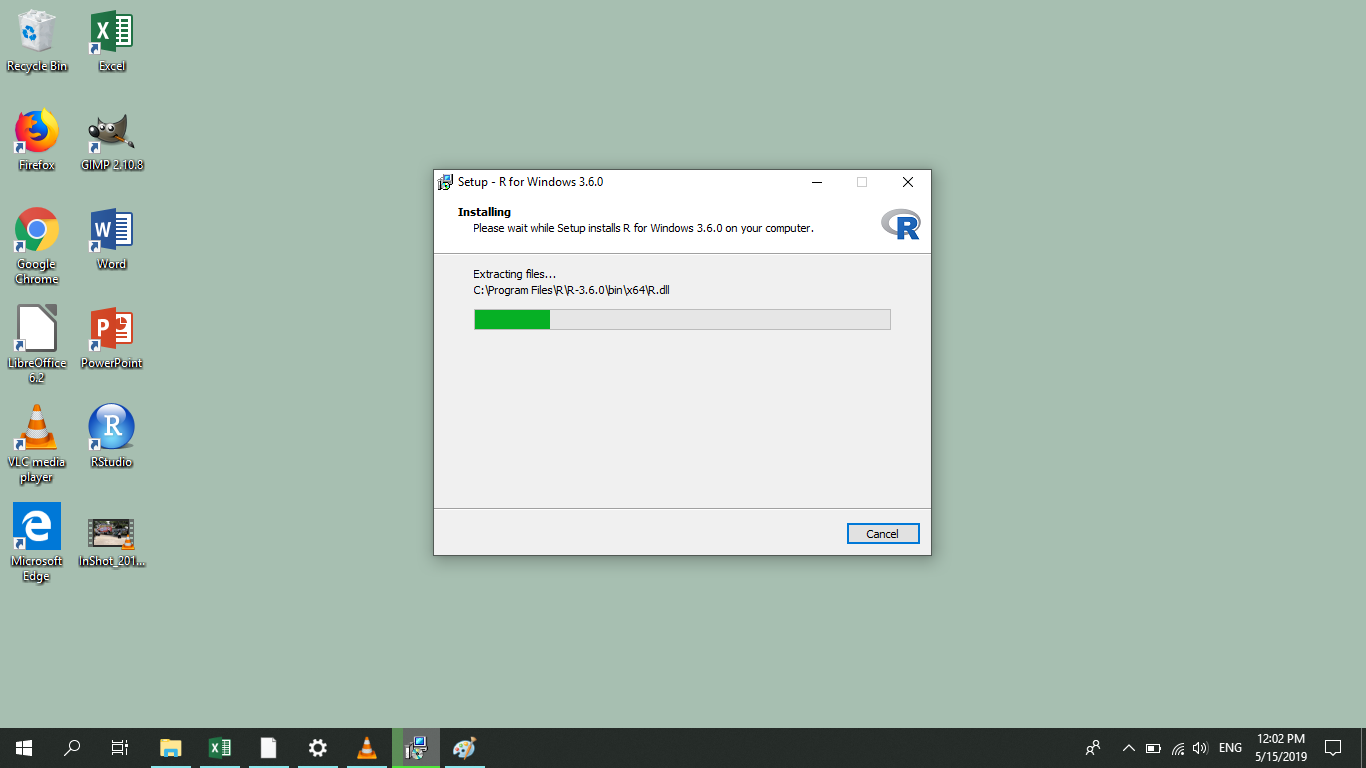
\includegraphics[width=0.9\linewidth]{Gambar/r-download/11} 

}

\caption{Kotak dialog terakhir setelah tomboh *Next* dan *Ok* dipilih}\label{fig:install-r-5}
\end{figure}

Untuk mempermudah pengerjaan menggunakan R, digunakan program Rstudio
IDE. Berikut adalah cara mengunduh Rstudio

\begin{enumerate}
\def\labelenumi{\arabic{enumi}.}
\tightlist
\item
  Pergi ke tautan
  \url{https://www.rstudio.com/products/rstudio/download/}
\item
  Cari tulisan ``Installers''
\item
  klik pada Rstudio 1.2.1335-Windows 7+ (64-bit)
\end{enumerate}

Memasang Rstudio IDE juga sama mudahnya dengan memasang program R.

\subsection*{Ubuntu 18.04}\label{ubuntu-18.04}
\addcontentsline{toc}{subsection}{Ubuntu 18.04}

Pengguna Ubuntu 18.04 dan Linux secara umum memiliki kelebihan yaitu
dapat menginstall program menggunakan terminal. Oleh karena itu, untuk
menginstall R dan Rstudio, pembaca hanya perlu melakukan
\textbf{Copy-Paste masing-masing script berikut secara baris per baris
di terminal.}

\begin{enumerate}
\def\labelenumi{\arabic{enumi}.}
\tightlist
\item
  Unduh dan pasang R
\end{enumerate}

\begin{Shaded}
\begin{Highlighting}[]
\FunctionTok{sudo}\NormalTok{ add-apt-repository }\StringTok{'deb https://cloud.r-project.org/bin/linux/ubuntu bionic-cran35/'}
\FunctionTok{sudo}\NormalTok{ apt-key adv --keyserver keyserver.ubuntu.com --recv-keys E298A3A825C0D65DFD57CBB651716619E084DAB9}
\FunctionTok{sudo}\NormalTok{ apt update}
\FunctionTok{sudo}\NormalTok{ apt install r-base r-base-dev}
\end{Highlighting}
\end{Shaded}

\begin{enumerate}
\def\labelenumi{\arabic{enumi}.}
\setcounter{enumi}{1}
\tightlist
\item
  Unduh dan pasang Rstudio
\end{enumerate}

\begin{Shaded}
\begin{Highlighting}[]
\FunctionTok{sudo}\NormalTok{ apt install gdebi}
\FunctionTok{wget}\NormalTok{ https://download1.rstudio.org/desktop/bionic/amd64/rstudio-1.2.1335-amd64.deb}
\FunctionTok{sudo}\NormalTok{ gdebi -i rstudio-1.2.1335-amd64.deb}
\end{Highlighting}
\end{Shaded}

\section{Penggunaan R}\label{penggunaan-r}

\subsection{Kalkulator}\label{kalkulator}

R pada bentuk sederhananya dapat dianggap sebagai sebuah kalkulator.
Kita dapat melaukan operasi dasar seperti 2 + 2 = 4.

\begin{Shaded}
\begin{Highlighting}[]
\DecValTok{2} \OperatorTok{+}\StringTok{ }\DecValTok{2} \OperatorTok{*}\StringTok{ }\DecValTok{10} \OperatorTok{/}\StringTok{ }\DecValTok{5} \OperatorTok{-}\StringTok{ }\DecValTok{10}
\end{Highlighting}
\end{Shaded}

\begin{verbatim}
## [1] -4
\end{verbatim}

\subsection{\texorpdfstring{Menyimpan objek dengan
\texttt{\textless{}-}}{Menyimpan objek dengan \textless{}-}}\label{menyimpan-objek-dengan--}

Dalam R, hasil dari suatu perhitungan dapat disimpan dalam sebuah objek.
Kita dapat menggunakan tanda \texttt{\textless{}-} untuk memasukkan
sesuatu ke dalam sebuah objek. Berikut adalah contoh.

\begin{Shaded}
\begin{Highlighting}[]
\NormalTok{x <-}\StringTok{ }\DecValTok{2} \OperatorTok{+}\StringTok{ }\DecValTok{2} \OperatorTok{*}\StringTok{ }\DecValTok{10} \OperatorTok{/}\StringTok{ }\DecValTok{5} \OperatorTok{-}\StringTok{ }\DecValTok{10}
\NormalTok{y <-}\StringTok{ }\DecValTok{9}
\NormalTok{z <-}\StringTok{ }\NormalTok{x}\OperatorTok{*}\NormalTok{y}

\KeywordTok{print}\NormalTok{(z)}
\end{Highlighting}
\end{Shaded}

\begin{verbatim}
## [1] -36
\end{verbatim}

\subsection{string}\label{string}

Selain angka, karakter atau \emph{string} juga dapat disimpan ke dalam
sebuah objek. String dalam R diawali dan diakhiri dengan tanda petik
(``)

\begin{Shaded}
\begin{Highlighting}[]
\NormalTok{nama <-}\StringTok{ "Wihelmus Wedo"}

\NormalTok{nama}
\end{Highlighting}
\end{Shaded}

\begin{verbatim}
## [1] "Wihelmus Wedo"
\end{verbatim}

\begin{Shaded}
\begin{Highlighting}[]
\KeywordTok{class}\NormalTok{(nama)}
\end{Highlighting}
\end{Shaded}

\begin{verbatim}
## [1] "character"
\end{verbatim}

\subsection{Vektor}\label{vektor}

Vektor dalam R dapat dipahami sebagai sekumpulan angka atau string.
Vektor memiliki sebuah kelas atau \emph{class}. Maksudnya, vektor dengan
kelas \emph{numeric} memiliki isi angka, dan vektor dengan kelas
\emph{character} memiliki isi string. Jika terdapat angka dan string
dalam suatu vektor, maka vektor tersebut menjadi vektor string. Vektor
dapat dibuat dengan menggunakan \texttt{c()}.

\begin{Shaded}
\begin{Highlighting}[]
\NormalTok{angka <-}\StringTok{ }\KeywordTok{c}\NormalTok{(}\DecValTok{1}\NormalTok{, }\DecValTok{2}\NormalTok{, }\DecValTok{3}\NormalTok{, }\DecValTok{4}\NormalTok{, }\DecValTok{5}\NormalTok{, }\DecValTok{6}\NormalTok{)}
\NormalTok{karakter <-}\StringTok{ }\KeywordTok{c}\NormalTok{(}\StringTok{"a"}\NormalTok{, }\StringTok{"b"}\NormalTok{, }\StringTok{"c"}\NormalTok{)}
\NormalTok{coba_ini <-}\StringTok{ }\KeywordTok{c}\NormalTok{(}\DecValTok{1}\NormalTok{, }\DecValTok{2}\NormalTok{, }\StringTok{"tiga"}\NormalTok{)}
\end{Highlighting}
\end{Shaded}

Selain \emph{numeric} dan \emph{character}, terdapat juga kelas lain
yang merupakan pengembangan. Dari kelas \emph{numeric}, pengembangannya
berupa

\begin{enumerate}
\def\labelenumi{\arabic{enumi}.}
\tightlist
\item
  \emph{integer}, yaitu vektor dengan bilangan bulat.
\item
  \emph{double}, yaitu vektor dengan bilangan riil.
\end{enumerate}

Sedangkan dari kelas \emph{character}, pengembangannya berupa

\begin{enumerate}
\def\labelenumi{\arabic{enumi}.}
\tightlist
\item
  \emph{factor}, yaitu vektor dengan adanya urutan pada elemen.
\item
  \emph{date}, yaitu vektor dengan pengembangan untuk penanggalan
  kalender.
\end{enumerate}

Secara umum, pengguna R disarankan untuk menggunakan kelas vektor yang
tepat. Sebagai contoh, angka seperti 1, 2, dan 3 disimpan dalam vektor
\emph{integer} dan tanggal di dalam vektor \emph{date}. Penggunaan yang
keliru seperti memasukkan sebuah tanggal ke dalam vektor angka atau
memasukkan bilangan riil ke dalam vektor \emph{factor} dan lain-lain,
dapat memberikan hasil yang membingungkan.

\begin{Shaded}
\begin{Highlighting}[]
\KeywordTok{class}\NormalTok{(angka)}
\end{Highlighting}
\end{Shaded}

\begin{verbatim}
## [1] "numeric"
\end{verbatim}

\begin{Shaded}
\begin{Highlighting}[]
\KeywordTok{class}\NormalTok{(karakter)}
\end{Highlighting}
\end{Shaded}

\begin{verbatim}
## [1] "character"
\end{verbatim}

\begin{Shaded}
\begin{Highlighting}[]
\KeywordTok{class}\NormalTok{(coba_ini)}
\end{Highlighting}
\end{Shaded}

\begin{verbatim}
## [1] "character"
\end{verbatim}

\subsection{\texorpdfstring{Tabel atau \emph{data
frame}}{Tabel atau data frame}}\label{tabel-atau-data-frame}

Pekerjaan di BPS biasanya dilakukan dalam sebuah tabel. Di dalam R,
tabel lebih dikenal dengan nama \emph{data frame}. Tabel atau \emph{data
frame} merupakan satu tingkat di atas vektor. Tabel memiliki baris dan
kolom. Kolom dalam sebuah tabel merupakan sebuah vektor. Dapat dikatakan
bahwa tabel merupakan kumpulan vektor yang memiliki panjang yang sama.
Berikut adalah salah satu \emph{data frame} bawaan dari R.

\begin{Shaded}
\begin{Highlighting}[]
\KeywordTok{head}\NormalTok{(beaver1)}
\end{Highlighting}
\end{Shaded}

\begin{verbatim}
##   day time  temp activ
## 1 346  840 36.33     0
## 2 346  850 36.34     0
## 3 346  900 36.35     0
## 4 346  910 36.42     0
## 5 346  920 36.55     0
## 6 346  930 36.69     0
\end{verbatim}

\chapter{Paket ggplot2}\label{ggplot2}

\section{Apa itu ggplot2?}\label{apa-itu-ggplot2}

\href{https://ggplot2.tidyverse.org/}{ggplot2} adalah paket yang
berfokus pada visualisasi statis. \texttt{ggplot2} adalah paket R yang
ditulis oleh Hadley Wickham. Bagian \emph{gg} dari ggplot2 merupakan
singkatan untuk \emph{Grammar of Graphics}, buku oleh Leland Wilkinson.
Paket \texttt{ggplot2} banyak digunakan pada bagian visualisasi data.

\texttt{ggplot2} mengaplikasikan suatu sistem pembuatan grafik yang
disebut dengan \emph{The Grammar of Graphics}. Pada sistem ini, gambar
dilihat dan dibentuk lapisan demi lapisan. Ada 3 hal yang penting dari
\texttt{ggplot2}, antara lain:

\begin{enumerate}
\def\labelenumi{\arabic{enumi}.}
\tightlist
\item
  \emph{data} dalam bentuk \emph{tidy},
\item
  \emph{aesthetics} seperti koordinat x, dan y, \emph{shape},
  \emph{color}, \emph{fill}, \emph{shape}, dan
\item
  \emph{geoms} yaitu objek geometrik seperti \emph{point}, \emph{bar},
  dan \emph{line}.
\end{enumerate}

Pengguna memberikan data, \emph{aesthetics}, dan jenis \emph{geoms} dan
\texttt{ggplot2} akan mengatur sisanya.

\section{\texorpdfstring{Pemasangan
\texttt{ggplot2}}{Pemasangan ggplot2}}\label{pemasangan-ggplot2}

\texttt{ggplot2} adalah salah satu bagian dari \emph{tidyverse}, paket R
yang berfokus pada analisis data. Memasang \texttt{tidyverse} secara
otomatis juga memasang \texttt{ggplot2}.

\begin{Shaded}
\begin{Highlighting}[]
\KeywordTok{install.packages}\NormalTok{(}\StringTok{"tidyverse"}\NormalTok{)}
\end{Highlighting}
\end{Shaded}

Namun, Jika pembaca ingin \textbf{hanya memasang paket ggplot2}, berikut
adalah cara untuk memasang paket \texttt{ggplot2}

\begin{Shaded}
\begin{Highlighting}[]
\KeywordTok{install.packages}\NormalTok{(}\StringTok{"ggplot2"}\NormalTok{)}
\end{Highlighting}
\end{Shaded}

\section{Penggunaan ggplot2}\label{penggunaan-ggplot2}

Dalam ggplot2, kita melihat plot atau grafik sebagai kumpulan
\textbf{lapisan} atau \emph{layer}. Banyak grafik yang dapat dihasilkan
menggunakan ide atau teori ini; \emph{scatter plot}, \emph{bar plot},
\emph{lolipop chart }, \emph{line chart}, \emph{heatmap}, \emph{map
plot} dan masih banyak lagi. Selain itu, ggplot2 adalah paket R,
sehingga banyak orang membuat paket-paket pendamping ggplot2 untuk
menghasilkan lebih banyak jenis plot; \emph{Treemap}, \emph{animation},
\emph{waffle chart}, dan masih banyak lagi.

\begin{Shaded}
\begin{Highlighting}[]
\KeywordTok{library}\NormalTok{(ggplot2)}
\end{Highlighting}
\end{Shaded}

\begin{verbatim}
## Registered S3 methods overwritten by 'ggplot2':
##   method         from 
##   [.quosures     rlang
##   c.quosures     rlang
##   print.quosures rlang
\end{verbatim}

\begin{Shaded}
\begin{Highlighting}[]
\CommentTok{#diamonds <- diamonds[1:1000,]}
\NormalTok{diamonds}
\end{Highlighting}
\end{Shaded}

\begin{verbatim}
## # A tibble: 53,940 x 10
##    carat cut       color clarity depth table price     x     y     z
##    <dbl> <ord>     <ord> <ord>   <dbl> <dbl> <int> <dbl> <dbl> <dbl>
##  1 0.23  Ideal     E     SI2      61.5    55   326  3.95  3.98  2.43
##  2 0.21  Premium   E     SI1      59.8    61   326  3.89  3.84  2.31
##  3 0.23  Good      E     VS1      56.9    65   327  4.05  4.07  2.31
##  4 0.290 Premium   I     VS2      62.4    58   334  4.2   4.23  2.63
##  5 0.31  Good      J     SI2      63.3    58   335  4.34  4.35  2.75
##  6 0.24  Very Good J     VVS2     62.8    57   336  3.94  3.96  2.48
##  7 0.24  Very Good I     VVS1     62.3    57   336  3.95  3.98  2.47
##  8 0.26  Very Good H     SI1      61.9    55   337  4.07  4.11  2.53
##  9 0.22  Fair      E     VS2      65.1    61   337  3.87  3.78  2.49
## 10 0.23  Very Good H     VS1      59.4    61   338  4     4.05  2.39
## # ... with 53,930 more rows
\end{verbatim}

Data \texttt{diamonds} -- data \emph{built in} dari paket ggplot2 --
digunakan sebagai contoh. Terdapat beberapa variabel dalam data diamond,
diantaranya

\begin{itemize}
\tightlist
\item
  \emph{carat} : berat dari berlian
\item
  \emph{cut} : kualitas potongan
\item
  \emph{color} : Warna berlian, dari J (terburuk) ke D (terbaik)
\item
  \emph{clarity} : Ukuran seberapa jernih suatu berlian
\item
  \emph{depth} : persentase kedalaman
\item
  \emph{table} : lebar dari ujung atas berlian relatif terhadap titik
  terlebar
\item
  \emph{price} : harga berlian dalam USD.
\item
  \emph{x} : panjang dalam milimeter
\item
  \emph{y} : lebar dalam milimeter
\item
  \emph{x} : kedalaman dalam milimeter
\end{itemize}

Informasi lainnya mengendai data \texttt{diamonds} dapat dilihat dengan
mengetik \texttt{?diamonds} pada \emph{console}. Misalkan kita ingin
mengetahui sebaran dari harga berlian. Dengan menggunakan informasi yang
tersedia, kita dapat mengidentifikasi lapisan \emph{data},
\emph{aesthetics}, dan \emph{geom} untuk gambar yang kita butuhkan.

\begin{enumerate}
\def\labelenumi{\arabic{enumi}.}
\tightlist
\item
  data : diamonds
\item
  aes : price
\item
  geom : histogram
\end{enumerate}

Dengan begitu, kita hanya perlu menyuruh R untuk membuat gambar.

\begin{Shaded}
\begin{Highlighting}[]
\NormalTok{ggdiamonds <-}\StringTok{ }\KeywordTok{ggplot}\NormalTok{(}\DataTypeTok{data =}\NormalTok{ diamonds, }\KeywordTok{aes}\NormalTok{(}\DataTypeTok{x =}\NormalTok{ price)) }\OperatorTok{+}
\StringTok{        }\KeywordTok{geom_histogram}\NormalTok{()}

\NormalTok{ggdiamonds}
\end{Highlighting}
\end{Shaded}

\begin{verbatim}
## `stat_bin()` using `bins = 30`. Pick better value with `binwidth`.
\end{verbatim}

\begin{center}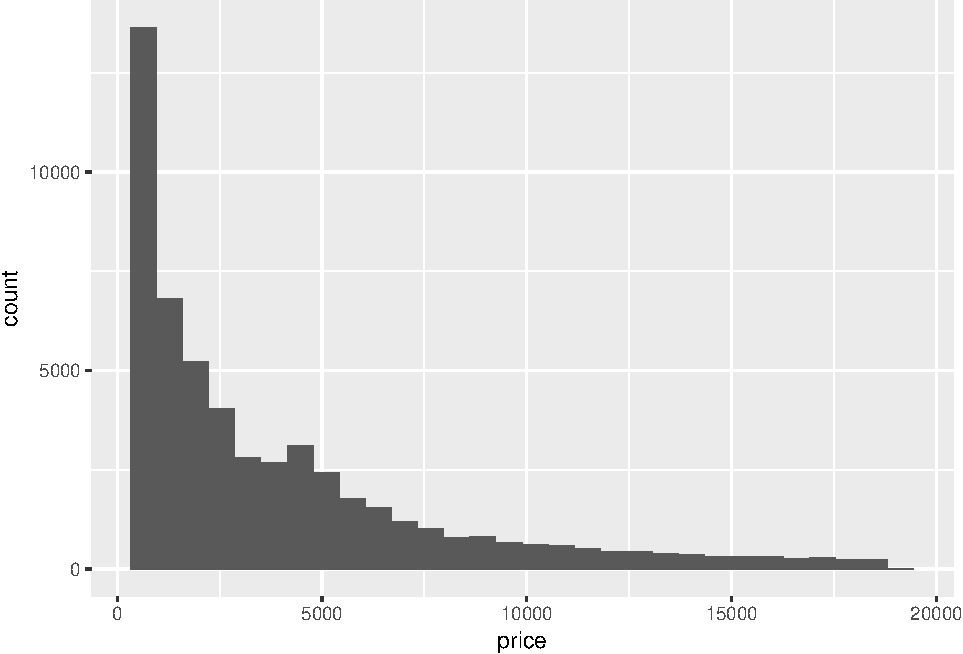
\includegraphics[width=0.9\linewidth]{Panduan_files/figure-latex/gg-diamonds-1} \end{center}

Pada fungsi \texttt{aes()}, kita memasukkan sumbu x sebab kita hanya
memerlukan 1 sumbu. Contoh berikutnya adalah menggunakan 2 sumbu.
Misalkan kita ingin melihat pola antara harga (\emph{price}) dan
kualitas potongan dari berlian (\emph{cut}). Arinyta kita akan membuat
\emph{scatter plot} antara \texttt{price} dan \texttt{cut}. Selama kita
dapat mengidentifikasi lapisan yang diperlukan:

\begin{enumerate}
\def\labelenumi{\arabic{enumi}.}
\tightlist
\item
  data : diamonds
\item
  aes : (x = price, y = cut)
\item
  geom : point
\end{enumerate}

Akan tetapi, kita juga ingin melihat pola antara harga har dan kualitas
potongan, dan juga warna. Oleh karena itu, kita membuatuhkan satu
\emph{aesthetic} lagi pada goem point.

\begin{Shaded}
\begin{Highlighting}[]
\NormalTok{ggprice <-}\StringTok{ }\KeywordTok{ggplot}\NormalTok{(}\DataTypeTok{data =}\NormalTok{ diamonds, }\KeywordTok{aes}\NormalTok{(}\DataTypeTok{x =}\NormalTok{ price, }\DataTypeTok{y =}\NormalTok{ carat)) }\OperatorTok{+}
\StringTok{        }\KeywordTok{geom_point}\NormalTok{(}\KeywordTok{aes}\NormalTok{(}\DataTypeTok{colour =}\NormalTok{ color))}

\NormalTok{ggprice}
\end{Highlighting}
\end{Shaded}

\begin{center}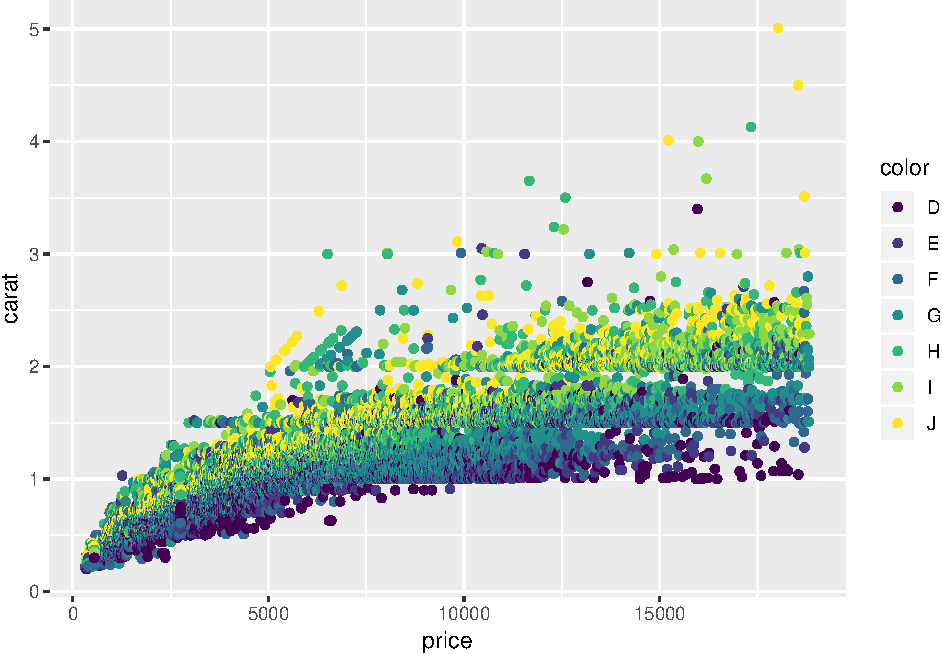
\includegraphics[width=0.9\linewidth]{Panduan_files/figure-latex/scatter-plot-1} \end{center}

\chapter{Tidyverse}\label{tidyverse}

\section{Apa itu tidyverse?}\label{apa-itu-tidyverse}

Ketika bekerja dengan data di dunia nyata seperti di BPS, paket
\texttt{ggplot2} saja tidak cukup. Paket \texttt{ggplot2} membutuhkan
\emph{tidy data} sebagai masukan, namun data yang dikumpulkan BPS
ataupun data yang berada di dunia nyata tidak selalu berada dalam bentuk
tersebut. Selain itu, terkadang dibutuhkan proses awal sebelum data
divisualisasikan. Proses ini dapat berupa agregasi berdasarkan variabel
tertentu, penyaringan terhadap kategori tertentu, ataupun menambahkan
variabel baru yang berperan dalam proses visualisasi. Untuk itu,
diperlukan paket-paket lainnya.

Hadley Wichkam dan komunitas R kemudian membuat paket-paket R lainnya
yang kemudian disebut sebagai \emph{tidyverse}. Tidyverse merupakan
koleksi dari paket yang bekerja kriteria \emph{tidy data}. Tidyverse
dibuat untuk memudahkan proses analisis data, mulai dari memasukkan data
(\emph{import data}), melakukan proses perapihan data (\emph{tidy}),
melakukan transformasi dan agregasi (\emph{transform}), visualisasi data
(\emph{visualization}), melakukan pemodelan (\emph{modelling}), hingga
menulis laporan (\emph{reporting}).

\section{Install tidyverse}\label{install-tidyverse}

Untuk menginstall paket \texttt{tidyverse} caranya sama dengan
menginstall paket \texttt{ggplot2}.

\begin{Shaded}
\begin{Highlighting}[]
\KeywordTok{install.package}\NormalTok{(}\StringTok{"tidyverse"}\NormalTok{)}
\end{Highlighting}
\end{Shaded}

Memasang \texttt{tidyverse} juga akan memasang paket-paket lain yang
tergabung dalam ekosistem tidyverse, sehingga waktu unduh dan pasang
akan lebih lama dibandingkan dengan waktu \texttt{ggplot2}

\section{Paket inti Tidyverse}\label{paket-inti-tidyverse}

Pada panduan ini penulis akan menjelaskan sedikit informasi mengenai
paket-paket inti dari tidyverse. Paket-paket ini disebut paket inti atau
\emph{core} sebab paket ini juga di \emph{attach} ketika
\texttt{tidyverse} di \emph{attach}. Paket \texttt{ggplot2} telah
dibahas pada bab sebelumnya sehingga tidak dibahas pada bagian ini.

\begin{Shaded}
\begin{Highlighting}[]
\KeywordTok{library}\NormalTok{(tidyverse)}
\end{Highlighting}
\end{Shaded}

\begin{verbatim}
## Registered S3 method overwritten by 'rvest':
##   method            from
##   read_xml.response xml2
\end{verbatim}

\begin{verbatim}
## -- Attaching packages ---------------------------------- tidyverse 1.2.1 --
\end{verbatim}

\begin{verbatim}
## v tibble  2.1.1       v purrr   0.3.2  
## v tidyr   0.8.3       v dplyr   0.8.0.1
## v readr   1.3.1       v stringr 1.4.0  
## v tibble  2.1.1       v forcats 0.4.0
\end{verbatim}

\begin{verbatim}
## -- Conflicts ------------------------------------- tidyverse_conflicts() --
## x dplyr::filter() masks stats::filter()
## x dplyr::lag()    masks stats::lag()
\end{verbatim}

\subsection{\texorpdfstring{\texttt{readr} dan
\texttt{tibble}}{readr dan tibble}}\label{readr-dan-tibble}

Paket \texttt{readr} digunakan dalam proses memasukkan data ke dalam
lingkungan R. \texttt{readr} menyediakan cara yang mudah untuk
memasukkan data yang \emph{rectangular} seperti \emph{csv} (\emph{comma
separated values}) dan \emph{tsv} (\emph{tab separated values}).

Paket \texttt{tibble} mungkin kurang populer dibandingkan paket inti
lainnya. \emph{Tibble} merupakan pengembangan dari \emph{data frame}.
Terdapat beberapa penambahan dan pengurangan fitur dari
\texttt{data.frame} yang dimiliki oleh sebuah \texttt{tbl\_df} yang
dapat membuat pekerjaan lebih mudah. Penambahan fitur seperti
memberitahu tipe atau \emph{class} dari semua kolom tabel serta
pengurangan fitur seperti meniadakan \emph{partial matching} diyakini
oleh para pembuat paket untuk membuat pekerjaan analisis data menjadi
lebih mudah. Tibble juga dapat melakukan hal lain namun hal tersebut
jarang penulis gali lebih dalam.

Data yang di\emph{import} menggunakan \texttt{readr} akan memiliki kelas
\texttt{tbl\_df}.

\subsection{\texorpdfstring{\texttt{tidyr}}{tidyr}}\label{tidyr}

Paket \texttt{tidyr} digunakan dalam proses perapihan data. Data rapi
atau \emph{tidy data} adalah bentuk data yang memenuhi \textbf{semua}
kriteria berikut.

\begin{enumerate}
\def\labelenumi{\arabic{enumi}.}
\item
  1(satu) variabel menempati 1(satu) kolom
\item
  1(satu) observasi atau individu menempati 1(satu) baris
\item
  1(satu) nilai atau \emph{value} menempati 1(satu) sel.
\end{enumerate}

Data rapi menunjukkan cara yang baku atau standar dalam menyimpan data.
Standar ini digunakan oleh semua paket dalam ekosistem Tidyverse.
Terdapat 2 fungsi yang sering digunakan dari paket \texttt{tidyr}, yaitu
\texttt{gather()} dan \texttt{spread()}.

\subsection{\texorpdfstring{\texttt{dplyr} dan
\texttt{\%\textgreater{}\%}}{dplyr dan \%\textgreater{}\%}}\label{dplyr-dan}

Paket \texttt{dplyr} adalah salah satu paket terpopuler (selain
\texttt{ggplot2}) dalam ekosistem tidyverse.

\begin{enumerate}
\def\labelenumi{\arabic{enumi}.}
\tightlist
\item
  \texttt{select()} \textbf{memilih} variabel/ kolom.
\item
  \texttt{filter()} \textbf{menyaring} tabel berdasarkan suatu kriteria.
\item
  \texttt{mutate()} \textbf{menambah} variabel/kolom yang merupakan
  fungsi dari variabel/kolom yang sudah ada.
\item
  \texttt{summarise()} atau \texttt{summarize()} \textbf{meringkas}
  tabel.
\item
  \texttt{arrange()} \textbf{mengurut} tabel berdasarkan variabel/kolom.
\end{enumerate}

Semua fungsi di atas digabungkan dengan \texttt{group\_by()} membuat
pengguna dapat menjalankan fungsi di atas \emph{berdasarkan kelompok}.
Lima fungsi di atas dibuat menggunakan kata kerja atau \emph{verbs}
untuk memudahkan pengguna memahami arti dari fungsi-fungsi tersebut.
Selain lima fungsi di atas ditambah \texttt{group\_by()}, \texttt{dplyr}
memiliki operator yang disebut sebagai \emph{foward pipe operator} atau
biasanya disingkat menjadi \emph{pipe}. Operator ini memiliki lambang
\texttt{\%\textgreater{}\%} dan dibaca \emph{kemudian} atau \emph{lalu}.

Pada umumnya, kode dibaca dari dalam ke luar (\emph{inside out}). Namun,
dengan menggunakan \texttt{\%\textgreater{}\%}, kode dapat dibaca dari
kiri ke kanan. Hal ini akan mempermudah seseorang untuk mengerti apa
yang sedang terjadi sehingga lebih mudah dimengerti.

Sebagai ilustrasi, perhatikan cerita pendek di bawah ini.

\begin{quote}
Hatori adalah seorang ninja.

Ia mendaki gunung, kemudian menuruni lembah, dan akhirnya mengarungi
samudra.
\end{quote}

Berdasarkan cerita pendek di atas, pada umumnya \textbf{script} akan
ditulis dalam satu baris, seperti berikut

\begin{Shaded}
\begin{Highlighting}[]
\NormalTok{hatori <-}\StringTok{ }\KeywordTok{as_ninja}\NormalTok{()}

\KeywordTok{mengarungi}\NormalTok{(}\KeywordTok{menuruni}\NormalTok{(}\KeywordTok{mendaki}\NormalTok{(hatori, gunung), lembah), samudra)}
\end{Highlighting}
\end{Shaded}

atau dalam bentuk yang agak condong ke dalam jika menggunakan
\emph{indent}.

\begin{Shaded}
\begin{Highlighting}[]
\NormalTok{hatori <-}\StringTok{ }\KeywordTok{as_ninja}\NormalTok{()}

\KeywordTok{mengarungi}\NormalTok{(}
  \KeywordTok{menuruni}\NormalTok{(}
    \KeywordTok{mendaki}\NormalTok{(hatori, gunung),}
\NormalTok{    lembah}
\NormalTok{  ),}
\NormalTok{  samudra}
\NormalTok{)}
\end{Highlighting}
\end{Shaded}

Untuk membaca \emph{script} di atas, diperlukan waktu yang relatif lebih
banyak dibandingkan ketika penulisan \emph{script} menggunakan
\texttt{\%\textgreater{}\%}. Berikut adalah \emph{script} yang sama jika
ditulis menggunakan \texttt{\%\textgreater{}\%}.

\begin{Shaded}
\begin{Highlighting}[]
\NormalTok{hatori <-}\StringTok{ }\KeywordTok{as_ninja}\NormalTok{()}

\NormalTok{hatori }\OperatorTok
\StringTok{  }\KeywordTok{mendaki}\NormalTok{(gunung) }\OperatorTok
\StringTok{  }\KeywordTok{menuruni}\NormalTok{(lembah) }\OperatorTok
\StringTok{  }\KeywordTok{mengarungi}\NormalTok{(samudra)}
\end{Highlighting}
\end{Shaded}

\subsection{\texorpdfstring{\texttt{stringr} dan
\texttt{forcats}}{stringr dan forcats}}\label{stringr-dan-forcats}

Paket \texttt{stringr} -- sesuai namanya -- digunakan ketika berurusan
dengan \emph{string} dalam proses analisis data. Di dalam dunia R,
\emph{string} juga dikenal dengan istilah \emph{character}.
Fungsi-fungsi dari paket \texttt{stringr} memiliki awalan \texttt{str\_}
pada nama.

\emph{forcats} adalah sebuah anagram untuk \emph{factors}. Sesuai dengan
namanya, \texttt{forcats} digunakan ketika berurusan \emph{factors}.
Mirip dengan \texttt{stringr}, fungsi-fungsi dalam paket ini memiliki
awalan \texttt{fct\_}.

\subsection{\texorpdfstring{\texttt{purrr}}{purrr}}\label{purrr}

Paket \texttt{purrr} dapat dikatakan memiliki tingkat kesulitan yang
lebih tinggi dibandingkan dengan paket inti lainnya. \texttt{purrr}
digunakan untuk mengimplementasikan \emph{functional programming}.

\section{Sumber ilmu lainnya}\label{sumber-ilmu-lainnya}

Tidyverse merupakan paket R yang luas sehingga panduan ini tidak cukup
menjelaskan semua paket di dalam ekosistem. Panduan ini juga hanya
menjelaskan sedikit informasi dari paket inti dari tidyverse. Masih
banyak informasi dari paket inti tidyverse yang penulis tidak bahas
dalam dokumen ini, terlebih mengenai paket-paket lain yang bukan paket
inti. Oleh karena itu, penulis berharap pembaca dapat mencari dan
membaca sendiri sumber-sumber lain mengenai tidyverse dan analisis data
menggunakan R.

\textbf{Tidyverse.org}

Tidyverse.org adalah situs yang khusus menjelaskan paket inti dari
tidyverse. Ini adlaah sumber nomor 1 bagi penulis ketika mengalami
masalah dengan paket inti tidyverse.

\textbf{stackoverflow.com}

StackOverFlow adalah sebuah forum dunia maya yang pada umumnya dihuni
oleh \emph{developer}. Dapat dibilang StackOverFlow ada forum tanya
jawab seputar hal-hal \emph{programming}. Banyak pertanyaan mengenai R
dan Rstudio yang ditanyakan di stackoverflow.

\textbf{community.rstudio.com},

Mirip seperti StackOverFlow, ini ada tempat bertanya khusus mengenai R
dan Rstudio. Forum ini dibuat oleh pihak Rstudio.

\textbf{youtube.co.id}

YouTube adalah situs berbagi video terbesar saat ini. Terdapat banyak
video tutorial maupun presentasi mengenai paket-paket dalam tidyverse.

\textbf{\#rstat}

Pengguna R memiliki komunitas di twitter. Komunitas ini biasanya
menggunakan tagar \#rstat memposting sesuatu tentang R.

\textbf{r/rstats}

Seperti di twitter, komunitas R juga terdapat di reddit. Komunitas R di
reddit berkumpul di \emph{subreddit} r/rstats.

\textbf{Google}

Google adalah \emph{search engine} yang paling besar. Mencari hal-hal
mengenai paket tidyverse merupakan hal mudah dengan menggunakan google.

\chapter{Project}\label{project}

Aktualisasi yang penulis lakukan bertujuan untuk meningkatkan
efektivitas dan efisiensi grafik dalam publikasi. Grafik yang efektif
adalah grafik yang mampu menyampaikan informasi. Konsumen dari grafik
yang efektif dapat dengan mudah mengerti tentang apa yang ditunjukkan
oleh suatu grafik. Grafik yang efisien adalah grafik yang dapat dibuat
dengan waktu yang lebih singkat serta dengan biaya yang sedikit mungkin.

Untuk meningkatkan efektivitas dan efisiensi grafik dalam publikasi,
penulis menuliskan 3 file.

\begin{enumerate}
\def\labelenumi{\arabic{enumi}.}
\item
  \texttt{ggplot\_theme.R} berisikan tema untuk objek ggplot2.
\item
  \texttt{ggplot\_skala.R} berisikan skala untuk sumbu x dan y
\item
  \texttt{ggplot\_pallete.R} berisikan \emph{palette} untuk
  \emph{aesthetic} \emph{color} dan \emph{fill}.
\end{enumerate}

\begin{Shaded}
\begin{Highlighting}[]
\KeywordTok{source}\NormalTok{(}\KeywordTok{here}\NormalTok{(}\StringTok{"Script/ggplot/ggplot_tema.R"}\NormalTok{))}
\KeywordTok{source}\NormalTok{(}\KeywordTok{here}\NormalTok{(}\StringTok{"Script/ggplot/ggplot_palette.R"}\NormalTok{))}
\KeywordTok{source}\NormalTok{(}\KeywordTok{here}\NormalTok{(}\StringTok{"Script/ggplot/ggplot_skala.R"}\NormalTok{))}

\NormalTok{gg_diamonds <-}\StringTok{ }\KeywordTok{ggplot}\NormalTok{(diamonds, }\KeywordTok{aes}\NormalTok{(}\DataTypeTok{x =}\NormalTok{ price)) }\OperatorTok{+}
\StringTok{  }\KeywordTok{geom_histogram}\NormalTok{(}\KeywordTok{aes}\NormalTok{(}\DataTypeTok{fill =}\NormalTok{ cut), }\DataTypeTok{binwidth =} \DecValTok{1000}\NormalTok{) }\OperatorTok{+}
\StringTok{  }\KeywordTok{scale_x_continuous}\NormalTok{(}\DataTypeTok{labels =} \KeywordTok{skl_rupiah}\NormalTok{(}\DataTypeTok{dari =} \StringTok{"rupiah"}\NormalTok{, }\StringTok{"ribu"}\NormalTok{)) }\OperatorTok{+}
\StringTok{  }\KeywordTok{scale_fill_manual}\NormalTok{(}\DataTypeTok{values =}\NormalTok{ plt5_}\DecValTok{04}\NormalTok{) }\OperatorTok{+}
\StringTok{  }\KeywordTok{theme_sbd}\NormalTok{()}

\NormalTok{gg_diamonds}
\end{Highlighting}
\end{Shaded}

\begin{center}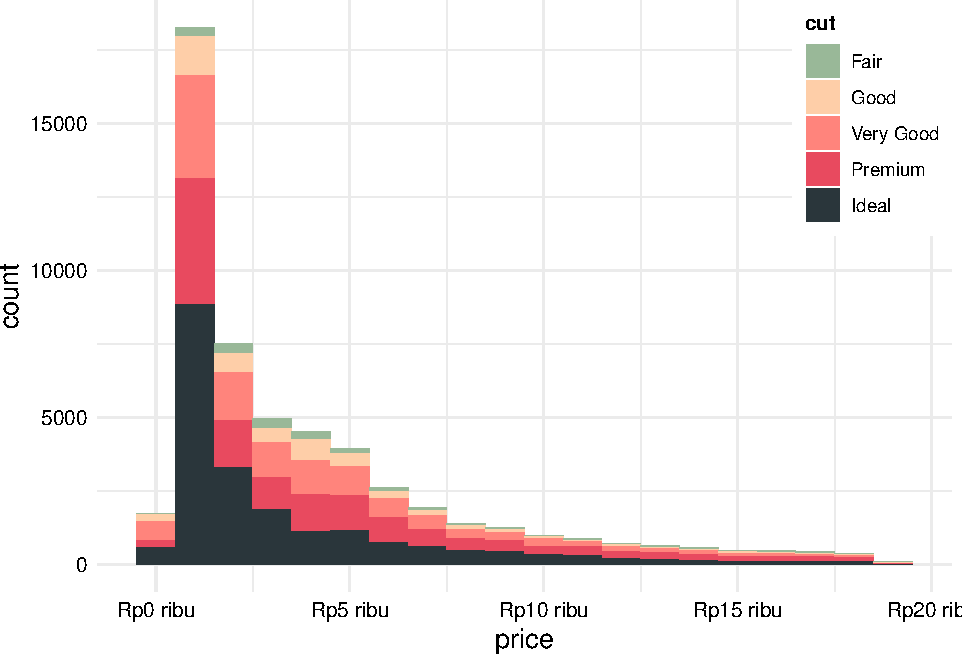
\includegraphics[width=0.9\linewidth]{Panduan_files/figure-latex/file-aktualisasi-1} \end{center}

Lumbung atau \emph{repository} aktualisasi tedapat pada
\url{https://git.bps.go.id/eus.wedo/sbd-grafik}. Cara mengunduh repo
tersebut terdapat pada README

\bibliography{book.bib,packages.bib}


\end{document}
